\pagebreak
\section{The ECCO Science Team 2025}
The ECCO Science team is a Consortium that is comprised of an international group of scientists across several institutions. The goal is to make the best possible estimates of ocean circulation and climate. Indeed, the ECCO products (state estimates) are multi-platform, multi-instrument synthesis products that integrate ocean and ice observations and models. ECCO science groups are listed below:


\vspace{.5cm}
Responsible for production of ECCO's central multi-decadal state estimate. Also developing estimation systems for ocean-ice interaction and global eddy-resolving models for ECCO's next generation estimate (\hyperlink{https://www.jpl.nasa.gov/}{Visit the JPL website}).

\vspace{.25cm}
\begin{center}
\begin{tabular}{ m{0.3\textwidth} m{0.33\textwidth}}
    \multicolumn{1}{c}{\textbf{Name}} & \multicolumn{1}{c}{\textbf{Institution}} \\ \hline
    Ian G. Fenty & NASA Jet Propulsion Laboratory, USA\\ \hline
    Ichiro Fukumori & NSAS Jet Propulsion Laboratory, USA \\ \hline
    Tong (Tony) Lee & NSAS Jet Propulsion Laboratory, USA \\ \hline
    Dimitris Menemenlis & NSAS Jet Propulsion Laboratory, USA \\ \hline
    Ou Wang & NSAS Jet Propulsion Laboratory, USA \\ \hline
    Hong Zhang & NSAS Jet Propulsion Laboratory, USA \\ \hline
\end{tabular}
\end{center}

\vspace{.25cm}
Responsible for MITgcm, the ocean general circulation model employed in all ECCO products (\hyperlink{http://web.mit.edu/}{Visit the MIT website}).

\vspace{.25cm}
\begin{center}
\begin{tabular}{m{0.3\textwidth} m{0.35\textwidth} }
    \multicolumn{1}{c}{\textbf{Name}} & \multicolumn{1}{c}{\textbf{Institution}} \\ \hline
    Jean-Michel Campin & Massachusetts Institute of Technology \\ \hline
    Gael Forget & Massachusetts Institute of Technology \\ \hline
    Chris Hill & Massachusetts Institute of Technology \\ \hline
    Diana Spiegel & Massachusetts Institute of Technology \\ \hline
    Carl Wunsch & Massachusetts Institute of Technology \\ \hline
\end{tabular}
\end{center}

\vspace{.25cm}
Responsible for ECCO adjoint model infrastructure. Also leading development of ocean-ice sheet parameterization and high-resolution estimation (\hyperlink{https://www.oden.utexas.edu/}{Visit the Oden Institute website at the University of Texas at Austin}).

\vspace{.25cm}
\begin{center}
\begin{tabular}{m{0.3\textwidth} m{0.32\textwidth} }
    \multicolumn{1}{c}{\textbf{Name}} & \multicolumn{1}{c}{\textbf{Institution}} \\ \hline
    Patrick Heimbach & University of Texas at Austin, USA \\ \hline
    An T. Nguyen & University of Texas at Austin, USA \\ \hline
    Helen Pillar & University of Texas at Austin, USA \\ \hline
    David Trossman & University of Texas at Austin, USA \\ \hline
    Nora Loose & University of Texas at Austin, USA \\ \hline
    Tim Smith & University of Texas at Austin, USA \\ \hline
    Ivana Escobar Casterlin & University of Texas at Austin, USA \\ \hline
\end{tabular}
\end{center}

\vspace{.25cm}
Responsible for development of new data sets and physics packages for the ECCO estimates. Also involved in assessing data and solution uncertainties and developing diagnostic tools for scientific analyses (\hyperlink{https://www.aer.com/}{Visit the Atmospheric and Environmental Research, Inc. website}).

\vspace{.25cm}
\begin{center}
\begin{tabular}{m{0.3\textwidth} m{0.46\textwidth} }
    \multicolumn{1}{c}{\textbf{Name}} & \multicolumn{1}{c}{\textbf{Institution}} \\ \hline
    Mengnan Zhao & Atmospheric and Environmental Research, Inc, USA \\ \hline
    Qiang Sun & Atmospheric and Environmental Research, Inc, USA \\ \hline
    Rui M. Ponte & Atmospheric and Environmental Research, Inc, USA \\ \hline
\end{tabular}
\end{center}

% \vspace{1cm}
\newpage
Leads development of regional high resolution estimation systems, including biogeochemistry (Southern Ocean [SOSE], California Current System, Equatorial Pacific, Gulf of Mexico) (\hyperlink{https://scripps.ucsd.edu/}{Visit the UC, San Diego website}).

\begin{center}
\begin{tabular}{m{0.3\textwidth} m{0.2\textwidth} }
    \multicolumn{1}{c}{\textbf{Name}} & \multicolumn{1}{c}{\textbf{Institution}} \\ \hline
    Bruce Cornuelle & UC, San Diego, USA \\ \hline
    Ganesh Gopalakrishnan  & UC, San Diego, USA \\ \hline
    Matt Mazloff  & UC, San Diego, USA \\ \hline
    Heriberto Vazquez Peralta  & UC, San Diego, USA \\ \hline
    Ariane Verdy  & UC, San Diego, USA \\ \hline
\end{tabular}
\end{center}

\vspace{.25cm}
Leads development of the global-ocean ECCO-Darwin biogeochemistry model.(\hyperlink{https://mlml.sjsu.edu/}{Visit the San José State University Moss Landing Marine Laboratories website}).

\begin{center}
\begin{tabular}{m{0.3\textwidth} m{0.25\textwidth} }
    \multicolumn{1}{c}{\textbf{Name}} & \multicolumn{1}{c}{\textbf{Institution}} \\ \hline
    Dustin Carroll  & UC, San Diego, USA \\ \hline 
\end{tabular}
\end{center}

\vspace{.25cm}
Leads development of 50+ year global ocean state estimation for studying longer-term climate variability and change [GECCO] (\hyperlink{https://www.oden.utexas.edu/}{Visit the University of Hamburg, Germany website}).

\begin{center}
\begin{tabular}{m{0.3\textwidth} m{0.34\textwidth} }
    \multicolumn{1}{c}{\textbf{Name}} & \multicolumn{1}{c}{\textbf{Institution}} \\ \hline
    Chevaly Albert Fernandez & University of Hamburg, Germany \\ \hline
    Armin Köhl & University of Hamburg, Germany \\ \hline
    Goukun Lyu & University of Hamburg, Germany \\ \hline
    Yulia Polkova & University of Hamburg, Germany \\ \hline
    Nuno Serra & University of Hamburg, Germany \\ \hline
    Detlef Stammer & University of Hamburg, Germany \\ \hline
\end{tabular}
\end{center}


\vspace{.25cm}
\begin{center}
Other institutions and team members involded in ECCO Science development:
\end{center}

\vspace{.25cm}
\begin{center}
\begin{tabular}{m{0.3\textwidth} m{0.45\textwidth} }
    \multicolumn{1}{c}{\textbf{Name}} & \multicolumn{1}{c}{\textbf{Institution}} \\ \hline
    Martin Losch & Alfred-Wegener-Institut (AWI), Germany\\ \hline
    Nils Hutter & Alfred-Wegener-Institut (AWI), Germany\\ \hline
    Madlen Kimmritz & Alfred-Wegener-Institut (AWI), Germany\\ \hline
    Geoffrey (Jake) Gebbie & Woods Hole Oceanographic Institution, USA\\ \hline
    Christopher Piecuch & Woods Hole Oceanographic Institution, USA\\ \hline
\end{tabular}
\end{center}


\pagebreak
\begin{center}
\begin{tabular}{m{0.25\textwidth} m{0.03\textwidth} m{0.25\textwidth} m{0.03\textwidth} m{0.25\textwidth}}
    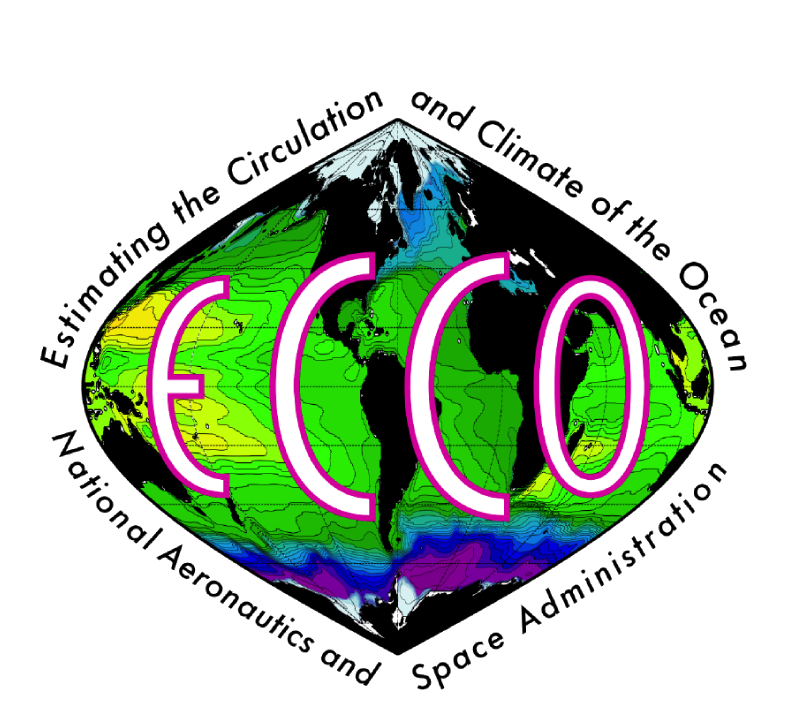
\includegraphics[width=0.3\textwidth]{../images/ecco_logo_800_726.png} & & 
\includegraphics[width=0.3\textwidth]{../images/logo_jpl.png} & & 
\includegraphics[width=0.3\textwidth]{../images/logo_mit.png}\\ 

    
\includegraphics[width=0.3\textwidth]{../images/logo_aer.png} & & 
\includegraphics[width=0.3\textwidth]{../images/logo_uta.png} & & 
\includegraphics[width=0.3\textwidth]{../images/ecco_teams_sjsu.png}\\

    
\includegraphics[width=0.3\textwidth]{../images/logo_uham.png} & & 
\includegraphics[width=0.3\textwidth]{../images/logo_sio.png} & & 
\includegraphics[width=0.3\textwidth]{../images/logo_whoi.png}\\ 
    
    
\includegraphics[width=0.3\textwidth]{../images/logo_awi.png} & & 
\includegraphics[width=0.2\textwidth]{../images/logo-podaac.png} & & 
\includegraphics[width=0.25\textwidth]{../images/logo-nasa.jpg}\\ 
\end{tabular}
\end{center}